% +--------------------------------------------------------------------+
% | Sample Chapter
% |
% | This file provides examples of how to
% | - insert a figure with a caption
% | - construct a table with a caption
% | - create subsections within the chapter
% | - insert a reference to a Figure or Table
% | - make a citation
% +--------------------------------------------------------------------+

\cleardoublepage

% +--------------------------------------------------------------------+
% | Replace "Chapter Title" below with the title of your chapter.  LaTeX
% | will automatically number the chapters.
% +--------------------------------------------------------------------+

\chapter{Introducción}
%\label{ch:Introducción}
\label{makereference}


% +--------------------------------------------------------------------+
% | Replace \section headings below with the title of your
% | subsections.  LaTeX will automatically number the subsections 1.1,
% | 1.2, 1.3, etc.
% +--------------------------------------------------------------------+

\section{Motivation}
\label{makereference1.1}

Cloud is a major word speaking about data compute in the last decade, we use cloud computing for processing every chunk of information from any source. 
If we move to Internet of Things field it is impossible not to put cloud computing in the same topic, cloud services are designed to provide easy, scalable access to applications, resources and services, and are fully managed by a cloud services provider.~\cite{cloud_def}  

Internet of things devices provide large amount of data, and we need cloud to process such kind of data, the Cloud of Things (CoT) term comes into play having devices connected directly to the cloud for perform complex operations with the generated data usually with Artificial Inteligence that is the perfect tool for creating smart tasks that would harness the inmense amount of information.
However cloud computing now faces several challenges to meet the more stringent performance requirements of many applications services, specially in terms of latency and bandwith.~\cite{IEE:Morabito:2017}

To solve those problems, Edge computing is a new paradigm that aims to bring data storage and computation closer to a selected location in order to improve response times and save data bandwitch, this consist on increasing the resources available on the edge adopting a platform that provide intermediate layers.
Thinking about these layers located at the edge make impossible the idea of having the same kind of datacenter that are being used for Cloud computing, this layer implies limited computational capabilities so one of the main problems to solve is to get similar cloud platforms into an Edge environment with certain compute power for processing data.
To solve this "compute power" problem the following resources are presented:

\begin{itemize}
  \item \textbf{Single Board computers or Minicomputers} that achieve high computing capacities reducing costs and size significantly.
  \item \textbf{Usb accelerators} devices that provides an Edge TPU as a coprocessor for your computer. It accelerates inferencing for artifical intelligence models.
\end{itemize}

Hardware part is covered, however there are too many things involving the current paradigm of cloud and edge computing that are essentials in order to build a proper architecture:

\textbf{Virtualization} is the capability of creating virtual machines that act like real ones, the creation of a virtual version of a device, this technology became mandatory in cloud and edge computing since the creation of automatic elastic services require to get rid of haphazard IT rooms, cables, and bulky hardware; reducing your overall IT overhead as well as management costs.~\cite{virt_def}.

Creation and management of these Virtual machines would be impossible without the existence of \textbf{hypervisors}, software which is responsible of controlling the virtual machine and provide a connection for the virtual resource and the real one.

\textbf{Virtual appliances} are Virtual Machine images, usually with a specific configuration, designed to run on a virtual platform. They are designed to reduce or eliminate the installation, configuration, and maintenance costs associated with running suites of software.~\cite{GEN:Virtualization:2010}

Having this in mind and knowing that in a near future there are going to be millions devices called things connected, the \textbf{IoT gateway} appears to serve as a bridge for connecting these things, send data to the cloud or participate with an edge approach, a way to implement this edge gateway might be build a virtual appliance that is situated close to the things. Figure ~\ref{figure1.1} show a representation of the concept.


\begin{figure}[h]%t=top, b=bottom, h=here
% \centering
    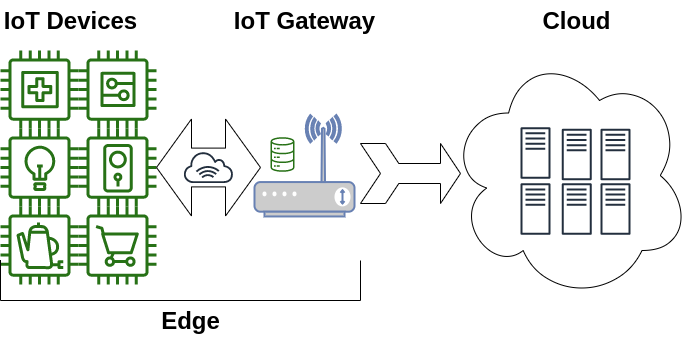
\includegraphics[width=6.5in]{figures/iot_gateway.png}
~\caption{IoT Gateway scheme}
\label{figure1.1}
\end{figure}

Some of the features that could supply the IoT gateway are the next:

\begin{itemize}
  \item communication bridge
  \item data storage, filter and aggregation
  \item device management and configuration
  \item Security 
  \item route data
\end{itemize}

\section{Objetivos}
\label{makereference1.2}

In this section, we refer back to text mentioned in
Section~\ref{makereference1.1} on page~\pageref{makereference1.1}.

\section{Estructura de la Memoria}
\label{makereference1.3}

Here's an example of a citation to a single
work.~\citet{CT:Weiner:1999} It's also possible to make multiple
citations.~\citet{CT:Phillips:1985, ARP:Loy:1974}
